\documentclass[11pt,a4paper]{article}

\usepackage{graphicx}
\usepackage{url}
\title{Different ways to connect to Raspberry Pi}
\author{e-Yantra Team}
\date{\today}

\begin{document}
	\maketitle
	\newpage
	\tableofcontents
	\newpage
	
	\flushleft
	In order to connect to a Raspberry Pi one can use one of the following methods:
	
	\section{HDMI to TV/PC monitor} 
	This is by far the simplest way to use the Raspberry Pi.
		\begin{figure}[h!]
			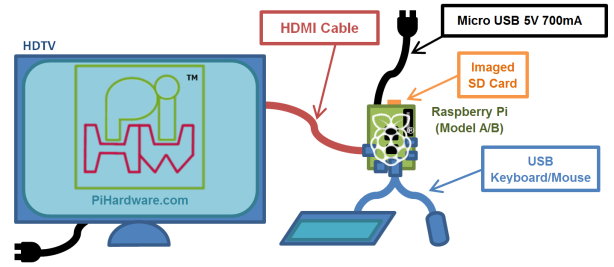
\includegraphics[scale=0.5]{tv.png}
			\centering
			\caption{[1]}
		\end{figure}
		     The setup includes connecting a digital TV/PC monitor to Raspberry Pi using HDMI cable (version 1.3a or above).
		     
		     \textbf{Advantages}
			     \begin{itemize}
			     	\item Simple quick setup
			     	\item Works directly out of the box
			     	\item Digital audio is provided as part of the HDMI connection
			     	\item High resolution display (up to 1080p)
			     \end{itemize}
			     
			  \textbf{Disadvantages}
				  \begin{itemize}
					  \item Requires a suitable screen to be available 
					  \item Not portable
				  \end{itemize}
				  
		\newpage
		\section{HDMI to DVI/VGA port of PC Monitor/TV}
		The HDMI connection can also be used to connect via a DVI connection, commonly available on newer monitors and digital TVs.
		\begin{figure}[h!]
			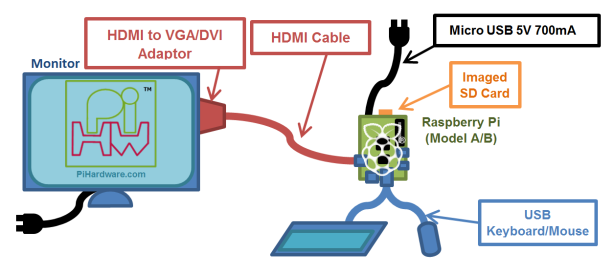
\includegraphics[scale=0.5]{pc.png}
			\centering
			\caption{[1]}
		\end{figure}
		
		The setup includes a TV (or screen) which has a DVI (or VGA) connection available and an HDMI to DVI adaptor (or HDMI to VGA adaptor). In this way we can connect a R-Pi to VGA monitor using a HDMI cable (version 1.3a or above).
		\textbf{Advantages}
		\begin{itemize}
			\item Simple quick setup
			\item Works directly out of the box
			\item HDMI to DVI adaptors are cheap
			\item High resolution display (up to 1080p)
		\end{itemize}
		
		\textbf{Disadvantages}
		\begin{itemize}
			\item Requires a suitable screen to be available 
			\item Not portable 
			\item Only supports analogue audio connection.
		\end{itemize}
		
		\newpage
		\section{Network cable to Laptop}
		In this method we connect the Pi to a laptop using a network cable(creating a localhost)
		\begin{figure}[h!]
			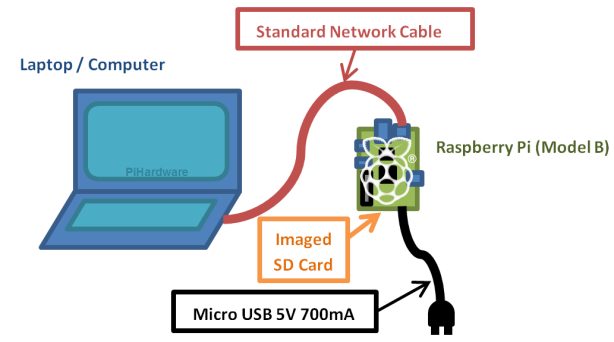
\includegraphics[scale=0.5]{nw.png}
			\centering
			\caption{[1]}
		\end{figure}
		
		In order to proceed to access R-Pi using this method follow these steps:
		\begin{enumerate}
			\item Find your laptop's(Windows 8 laptop) network settings in the following way:
			\begin{itemize}
				\item From the Start Menu, run the “Control Panel”.
				\item Open "Network and Internet" , then “Network and Sharing Center” and click on “Change adapter settings” on the left side.
				\item Find the item which relates to your Wired network adaptor (by default this is usually called “Local Area Connection”).
				\item Right-click on it and open “Properties”.
				\item Select the item which is called “Internet Protocol (TCP/IP)” or “Internet Protocol Version 4 (TCP/IPv4)” if there are two (the other is Version 6), and open the “Properties”.
				\item Hopefully, the IP Address will be set to “Obtain an IP address automatically”.  If not don’t worry, just take a note of the IP address and Subnet Mask set here.
			\end{itemize}
			\item Setting up Raspberry Pi's IP address
			\begin{itemize}
				\item Ensure the Raspberry Pi is powered off, and remove the SD-Card.
				\item Insert the SD-Card into a card reader and plug it into your laptop.
				\item Find the drive and you should find several files on the Card (note it a lot smaller than you’d expect since it is only the boot section of the Card (the rest is hidden)).
				\item Make a copy of cmdline.txt and rename it cmdline.normal
				\item Edit cmdline.txt and add the IP address at the end (be sure you don’t add any extra lines).
				\item For network settings where the IP address is obtained automatically, use an address in the range 169.254.X.X (169.254.0.0 – 169.254.255.255) say 169.254.0.2.
				For network settings where the IP address is fixed, use an address which matches the laptop/computers address except the last digit say 192.168.0.2
				\item Ensure you take note of this IP address (you will need it every time you want to directly connect to the Raspberry Pi).
				\item Make new copy of cmdline.txt and rename it cmdline.direct
				\item To swap between configurations, just replace cmdline.txt with either cmdline.normal or cmdline.direct 
				\item Return the card to the Raspberry Pi. Attach the network cable attached to both the computer and Raspberry Pi and power up.
			\end{itemize}
		\end{enumerate}
		Now u can start using the Pi directly.	
	    
	    \section{USB Wifi Dongle to Router}
	    
	    In this method we connect Wifi Dongle to R-Pi. As a result the R-Pi gets connected to wireless network and a user can access it using the IP address of R-Pi.
	    
	    In order to start using wireless network one needs to edit some files on R-Pi.For more information regarding this kindly refer \textit{Experiments} section of  \url{https://github.com/eyantrainternship/eYSIP_2015_RaspberryPi-Development-Board/tree/master/2_Establishing%20network%20connection%20and%20SSH%20connection}
	    
	    \vspace{0.3cm}	
	    \textbf{Advantages}
	    \begin{itemize}
	    	\item Simple quick setup
	    	\item Requires no separate monitor for setup
	    	\item No need of HDMI cable
		    \item High resolution display (up to 1080p)
		    \item Offers remote connectivity
	    \end{itemize}
	    
	    \textbf{Disadvantages}
	    \begin{itemize}
	    	\item SSH connection is slow if the network is weak 
	    \end{itemize}
	    
	    
	
	\vspace{0.5cm}
	\section{References}
	\begin{enumerate}
		\item https://pihw.wordpress.com/guides/guide-to-ways-to-connect-to-a-raspberry-pi/
	\end{enumerate}
\end{document}



